\section{Story Splitting}
In the following section the concept of story splitting is introduced which can be used for component identification.

The acronym INVEST helps to remember a widely accepted set of criteria, or checklist, to assess the quality of a user story. If the story fails to meet one of these criteria, the team may want to reword it, or even consider a rewrite (which often translates into physically tearing up the old story card and writing a new one).

\begin{description}
	\item [I]ndependent (of all others)
	\item [N]egotiable (not a specific contract for features)
	\item [V]aluable (or vertical)
	\item [E]estimable (to a good approximation)
	\item [S]mall (so as to fit within an iteration)
	\item [T]estable (in principle, even if there isn't a test for it yet)
\end{description}

The following Figure \ref{fig:storysplitting} displays nine splitting patterns for userstories.

\begin{figure}[H]
  \center
  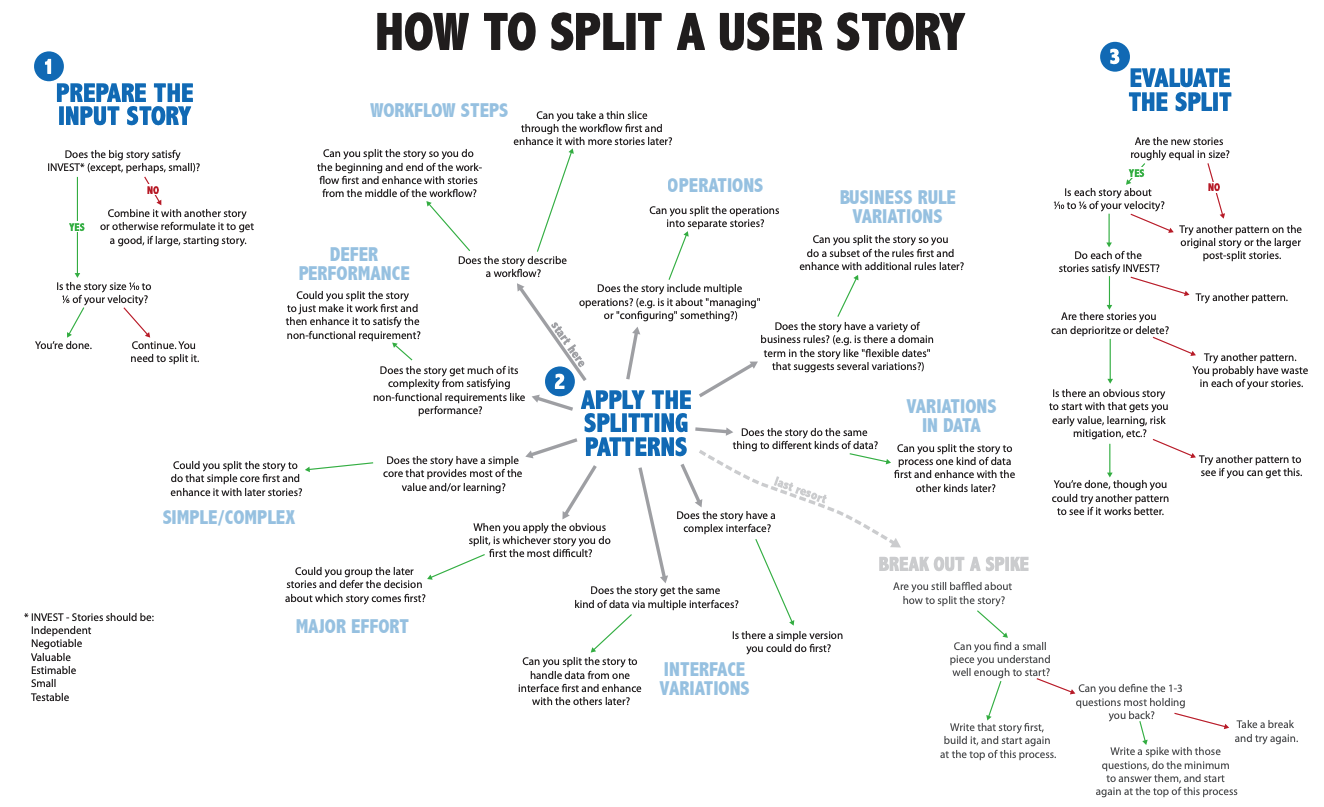
\includegraphics[width=\textwidth]{splitauserstory}
  \caption{Split a User Story}
  \label{fig:storysplitting}
\end{figure}

\paragraph{Example Story Splitting} \hfill \\
\textit{User Story:} As a veterinarian working for the Pet Clinic, I want to schedule visits of pets and their owners so that I can heal as many animals as possible and send invoices to their owners.

\begin{table}[H]
\centering
	\begin{tabular}{|l|l|l|}
	\hline
	\textbf{Pattern}          & \textbf{Story Element}                                                                                                                                         & \textbf{Impact on Architecture}                                                                                                                                                        \\ \hline
	Pattern 1: Workflow Steps & 
	\begin{tabular}[c]{@{}l@{}}A visit must be requested, \\ scheduled, executed, documented, \\ billed, invoices must be created, \\ sent, monitored\end{tabular} &
	\begin{tabular}[c]{@{}l@{}}Request visit etc.; at least one new\\ \\ input view per step/story; business\\ logic to assign vets to slots and\\ patents (owners with pets)\end{tabular} \\ \hline
\end{tabular}
\end{table}

\section{Component Modeling}
 A candidate component is an architectural element in the logical viewpoint grouping related responsibilities that jointly satisfy one or more (non-)functional requirements so that design and implementation work can be planned and component realization decisions can be made.
 
 The C4 component diagram takes a logical view point. It is initialized during solution strategy, populated in project iterations and well suited to show layers and candidate components. 

\begin{figure}[H]
  \center
  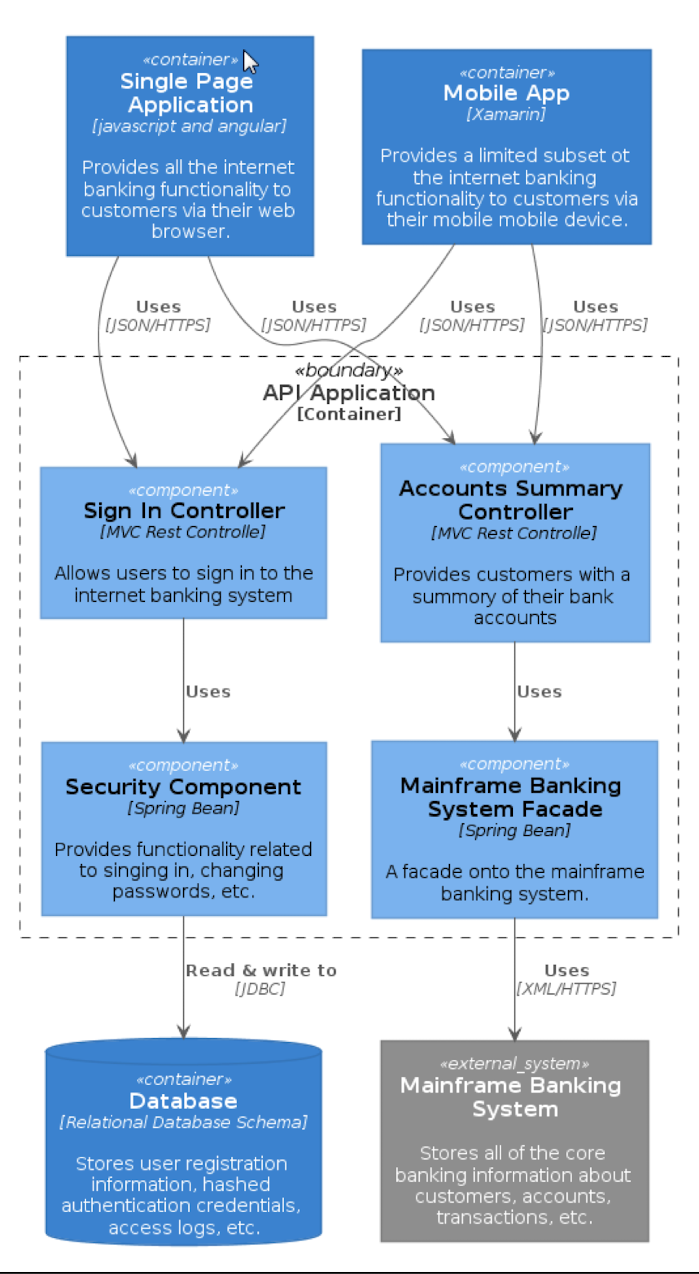
\includegraphics[width=0.45\textwidth]{componentdiagram}
  \caption{Sample Component Diagram}
\end{figure}

\subsection{C4 Notation}

\paragraph{Diagrams}
\begin{itemize}
	\item Every diagram should have a title describing the diagram type and scope (e.g. "System Context diagram for My Software System").
	\item Every diagram should have a key/legend explaining the notation being used (e.g. shapes, colours, border styles, line types, arrow heads, etc).
	\item Acronyms and abbreviations (business/domain or technology) should be understandable by all audiences, or explained in the diagram key/legend.
\end{itemize}

\paragraph{Elements}
\begin{itemize}
	\item The type of every element should be explicitly specified (e.g. Person, Software System, Container or Component).
	\item Every element should have a short description, to provide an "at a glance" view of key responsibilities.
	\item Every container and component should have a technology explicitly specified.
\end{itemize}

\paragraph{Relationship}
\begin{itemize}
	\item Every line should represent a unidirectional relationship.
	\item Every line should be labelled, the label being consistent with the direction and intent of the relationship (e.g. dependency or data flow). Try to be as specific as possible with the label, ideally avoiding single words like, "Uses".
	\item Relationships between containers (typically these represent inter-process communication) should have a technology/protocol explicitly labelled.
\end{itemize}

\subsection{ZIOs Component Identification Algorithm}
\textbf{Output:} Refined requirements and domain model, C4 diagrams, CRC cards

\begin{enumerate}
	\item First iteration: Find Candidate Components (\textbf{CanCons})
	\begin{enumerate}
		\item One channel component per primary actors (user/system) in context
		\item One component per layer per feature (story) and domain model partition
		\item One adapter component per backend system appearing in context
	\end{enumerate}
	\item CRC brainstorming or workshop (to find responsibilities, collaborators)
	\item Starting in second iteration: Architectural Refactoring (of CRC cards)
	\begin{itemize}
		\item Address quality concerns such as security and management
		\item List potential realiziation technologies
		\item Run a sanity/completeness check
	\end{itemize}
\end{enumerate}



